\documentclass[letterpaper,11pt]{article}

\usepackage{latexsym}
\usepackage[empty]{fullpage}
\usepackage{titlesec}
\usepackage{marvosym}
\usepackage[usenames,dvipsnames]{color}
\usepackage{verbatim}
\usepackage{enumitem}
\usepackage[hidelinks]{hyperref}
\usepackage{fancyhdr}
\usepackage[english]{babel}
\usepackage{tabularx}
\usepackage{fontawesome5}
\usepackage{multicol}
\setlength{\multicolsep}{-3.0pt}
\setlength{\columnsep}{-1pt}
\input{glyphtounicode}

%new packages

\usepackage{fontenc}
\usepackage{amsmath}
\usepackage{amssymb}
\usepackage{graphicx}



%----------FONT OPTIONS----------

\pagestyle{fancy}
\fancyhf{} % clear all header and footer fields
\fancyfoot{}
\renewcommand{\headrulewidth}{0pt}
\renewcommand{\footrulewidth}{0pt}

% Adjust margins
\addtolength{\oddsidemargin}{-0.6in}
\addtolength{\evensidemargin}{-0.5in}
\addtolength{\textwidth}{1.19in}
\addtolength{\topmargin}{-.7in}
\addtolength{\textheight}{1.4in}

\urlstyle{same}

\raggedbottom
\raggedright
\setlength{\tabcolsep}{0in}

% Sections formatting
\titleformat{\section}{
  \vspace{-4pt}\scshape\raggedright\large\bfseries
}{}{0em}{}[\color{black}\titlerule \vspace{-5pt}]



% Ensure that generate pdf is machine readable/ATS parsable
\pdfgentounicode=1

%-------------------------
% Custom commands
\newcommand{\resumeItem}[1]{
  \item\small{
    {#1 \vspace{-2pt}}
  }
}

\newcommand{\classesList}[4]{
    \item\small{
        {#1 #2 #3 #4 \vspace{-2pt}}
  }
}

\newcommand{\resumeSubheading}[4]{
  \vspace{-2pt}\item
    \begin{tabular*}{1.0\textwidth}[t]{l@{\extracolsep{\fill}}r}
      \textbf{#1} & \textbf{\small #2} \\
      \textit{\small#3} & \textit{\small #4} \\
    \end{tabular*}\vspace{-7pt}
}

\newcommand{\resumeSubSubheading}[2]{
    \item
    \begin{tabular*}{0.97\textwidth}{l@{\extracolsep{\fill}}r}
      \textit{\small#1} & \textit{\small #2} \\
    \end{tabular*}\vspace{-7pt}
}

\newcommand{\resumeProjectHeading}[2]{
    \item
    \begin{tabular*}{1.001\textwidth}{l@{\extracolsep{\fill}}r}
      \small#1 & \textbf{\small #2}\\
    \end{tabular*}\vspace{-7pt}
}


\newcommand{\resumeSubItem}[1]{\resumeItem{#1}\vspace{-4pt}}

\renewcommand\labelitemi{$\vcenter{\hbox{\tiny$\bullet$}}$}
\renewcommand\labelitemii{$\vcenter{\hbox{\tiny$\bullet$}}$}

\newcommand{\resumeSubHeadingListStart}{\begin{itemize}[leftmargin=0.0in, label={}]}
\newcommand{\resumeSubHeadingListEnd}{\end{itemize}}
\newcommand{\resumeItemListStart}{\begin{itemize}}
\newcommand{\resumeItemListEnd}{\end{itemize}\vspace{-5pt}}

\begin{document}
\fontfamily{cmr}\selectfont
\begin{center}
\parbox{3.0cm}{%
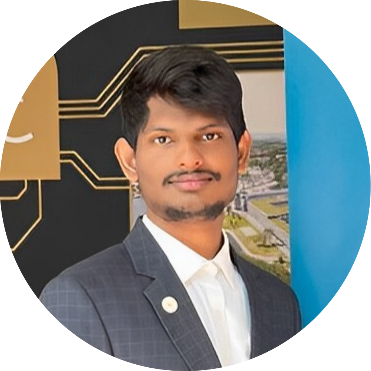
\includegraphics[width=2.7cm,clip]{images/resume_pic_m.png}}
}
\parbox{\dimexpr\linewidth-3.8cm\relax}{
\vspace{-20pt}
\begin{tabularx}{\linewidth}{L r} \\
    {\Huge \scshape  Venkata Sai Yakkshit Reddy Asodi}~
    \href{https://www.cedzlabs.com/yakkshit}{\vspace{1pt}}\\
      Mainz, Germany. \\ \vspace{1pt}
     \small \raisebox{-0.1\height}\faPhone\ +91 8179936156 ~ \href{mailto:saiyakkshit2001@gmail.com}{\raisebox{-0.2\height}\faEnvelope\  {saiyakkshit2001@gmail.com}} ~ 
    \href{https://linkedin.com/in/yakkshit/}{\raisebox{-0.2\height}\faLinkedin\ {yakkshit}}  ~
    \href{https://yakkshit.com/}{\raisebox{-0.2\height}\faGlobe\ {yakkshit.com}}  ~
    \href{https://github.com/yakkshit}{\raisebox{-0.2\height}\faGithub{ yakkshit}}
    \vspace{-8pt}
\end{tabularx}
}
\end{center}

\vspace{-23pt}
%-----------EDUCATION-----------
\href{https://www.yakkshit.com/#details}{\section{Summary \faLink}
Versatile Flutter Developer with strong expertise in mobile and web development, specializing in creating responsive cross-platform applications. Proven track record in developing AI-integrated solutions and optimizing application performance. Experience in architectural design and implementation of user-friendly interfaces. Fluent in German (B2 level) with a passion for collaborative development and maintaining scalable codebases.}

%-----------PROGRAMMING SKILLS-----------
\section{\href{https://www.linkedin.com/in/yakkshit/details/skills/}{Technical Skills} \faLink}
\begin{itemize}[leftmargin=0.15in, label={}]
\small{\item{
\textbf{Mobile Development - }{Flutter, Dart, Mobile UI/UX Design, Cross-platform Development} \\
\textbf{Frontend - }{React Native, React.js, Vue.js} \\
\textbf{Testing - }{Unit Testing, Integration Testing, Test-Driven Development} \\
\textbf{Tools - }{Git, RESTful APIs, Firebase, CI/CD} \\
\textbf{Cloud \& DevOps - }{AWS, Azure, Docker}\\
}}
\end{itemize}
\vspace{-10pt}

%-----------EXPERIENCE-----------
\section{Experience \faLinkedin}

\resumeSubHeadingListStart

\resumeSubheading
{\large Circleup AG \faBuilding}{December 2023 -- July 2024}
{Senior Mobile Developer}{\faMapMarker \hspace{0.1cm} Zurich, Switzerland}\\
\vspace{10pt}
\textbf{Responsibilities:}
\resumeItemListStart
\vspace{-10pt}
\resumeItem{Led the development of cross-platform mobile applications using Flutter and Dart, implementing complex UI components and ensuring optimal performance across iOS and Android platforms.}
\resumeItem{Architected and implemented real-time data synchronization features for AI-driven services, achieving 40\% improvement in app performance and 99\% crash-free sessions.}
\resumeItemListEnd
\vspace{-3pt}
\textbf{Environment:}\emph{Flutter, Dart, Firebase, RESTful APIs, Unit Testing}

\resumeSubheading
{Cedzlabs \faBuilding}{March 2023 -- July 2024}
{Mobile Application Developer}{\faMapMarker \hspace{0.1cm} Germany}\\
\vspace{10pt}
\textbf{Responsibilities:}
\vspace{-10pt}
\resumeItemListStart
\resumeItem{Developed and maintained cross-platform applications using Flutter, implementing comprehensive testing strategies and collaborating with design teams to create intuitive user interfaces.}
\resumeItemListEnd
\vspace{-3pt}
\textbf{Environment:}\emph{Flutter, Dart, Material Design, Git, Integration Testing}

\resumeItem{\textbf{\href{https://linkedin.com/in/yakkshit}{View additional experience on LinkedIn}}}
\vspace{-5pt}

%-----------PROJECTS-----------
\section{Projects \faGithub}
\vspace{-5pt}
\resumeSubHeadingListStart
\resumeProjectHeading
{\textbf{\href{https://ui.cedzlabs.com/resume}{Customer Feedback Analytics App}} $|$ \emph{Flutter, Dart, AI Integration}}{2023}\\
\vspace{6pt}
\textbf{Description:}
\vspace{-5pt}
\resumeItemListStart
\resumeItem{Engineered a Flutter-based mobile application for analyzing customer feedback using AI algorithms. Implemented real-time data visualization, offline functionality, and seamless backend integration. Achieved significant performance optimization through efficient state management and caching strategies.}
\resumeItemListEnd
\vspace{4pt}
\textbf{Tools:}\emph{Flutter, Dart, Firebase, Unit Testing, Provider State Management}
\vspace{-10pt}

\resumeProjectHeading
{\href{https://yakkshit.com}{\textbf{Cross-platform Portfolio App}} $|$ \emph{Flutter, AWS}}{2023}\\
\vspace{6pt}
\textbf{Description:}
\vspace{-5pt}
\resumeItemListStart
\resumeItem{Developed a feature-rich portfolio application using Flutter, showcasing expertise in custom animations, state management, and responsive design. Implemented comprehensive testing suite and automated deployment pipeline.}
\resumeItemListEnd
\vspace{4pt}
\textbf{Tools:}\emph{Flutter, Dart, AWS, Integration Testing}
\vspace{-12pt}

%-----------INVOLVEMENT---------------
\section{Achievements / Extracurricular / Contributions}
\resumeSubHeadingListStart
\resumeItemListStart
\resumeItem{Advanced Flutter Development Certification from Google}
\resumeItem{Regular contributor to Flutter open-source projects and community forums}
\resumeItem{Published technical articles on Flutter best practices and performance optimization}
\resumeItemListEnd

\resumeSubHeadingListEnd
\textbf{Strengths: }\emph{Mobile Architecture Design, Cross-platform Development, Problem-solving, Team Collaboration} \\
\textbf{Languages: }\emph{German - B2 $|$ English - Fluent $|$ Telugu - Native $|$ Hindi - Fluent $|$ Swedish - Elementary}

\vspace{10pt}
\end{document}